% Last Modification:
% @author AUTHOR_NAME
% @date TODAY_DATE

\chapter{General Description}
\label{chap:general_description}

In the context of the \msrmessir method, the information provided in this section is intended to present the system for which the \msrmessir analysis is provided. The content of this section is made accordingly to the requirements elicitation document that might have been done during the project but also adapted coherently in order to be an abstract introduction to the \msrmessir analysis.

\section{Domain Stakeholders}
\label{sec:icrash-gendescr-stakeholders}

All stakeholders of the system are detailed in this section. After a brief description of a
stakeholder, its objectives are first stated. Thereafter, the responsibilities of
the stakeholder are detailed which help to achieve the stakeholder objectives to a certain
degree. While the objectives characterize the general problems addressed by the \msricrash system,
the responsibilities describe concrete actions that are expected from a stakeholder. Some of
these responsibilities can be traced looking at the use case described in Section \ref{sec:icrash-gendescr-usecasemodel},and hence must be supported by the \msricrash  system. 
All stakeholders listed in this section have an interest in the system or are affected
by the system in some way, but only a subset of the stakeholders are directly involved in the use
cases described.
Let us remind that use case diagrams or descriptions are not \msrmessir analysis phase mandatory outputs. They are proposed as informal means to help understanding the semantics of the system specification made of the mandatory analysis models, which provide a complete executable specification.

\subsection{Communication Company}
A Communication Company is a company that has the capacity to ensure communication of information between its customers and the \msricrash system. 
The objectives of a Communication Company are:
\begin{itemize}
  \item to be able to deliver any SMS sent by any human to the \msricrash's phone number.
  \item to be able to transmit SMS messages from the ABC company that owns the \msricrash system to any human having a SMS compatible device accessible using a phone number.
\end{itemize}
\vspace{0.5cm}

In order to achieve these objectives, the responsibilities of a Communication Company are:
\begin{itemize}
  \item ensure confidentiality and integrity of the information sent by a human to the \msricrash system or from the system to a human.
  \item to be always available and reliable.
\end{itemize}

\subsection{Humans}
A human is any person who considers himself related to a car crash either as a witness, a victim or an anonymous person. The objectives of a human are:
\begin{itemize}
  \item inform the \msricrash system about the crisis situation he detected.
  \item be sure that the ABC company has been informed about the situation.
  \item to be informed about the situation of the crisis he his related to as a victim or witness.
\end{itemize}
\vspace{0.5cm}

In order to achieve these objectives, the responsibilities of a human are:
\begin{itemize}
  \item to provide has much details as possible, even tho these details might
  contain errors, concerning the crisis to the ABC company.
  \item to declare a crisis only if the crisis is real.
  \item to have access to the SMS compatible communication device he used to communication with the \msricrash system.
\end{itemize}

\subsection{Coordinators}
A coordinator is a employee of the ABC company being responsible of handling one or several crisis. The objectives of a coordinator are:
\begin{itemize}
  \item to securely monitor the existing alerts and crisis.
  \item to securely manage alerts and crisis until their termination.
\end{itemize}
\vspace{0.5cm}

In order to achieve these objectives, the responsibilities of a coordinator are:
\begin{itemize}
  \item to be capable to determine how an alert received should be considered.
  \item to be available to react to requests to handle alerts and crisis.
  \item to be autonomous in handling crisis and to report on its handling.
  \item to be able to decide when a crisis or an alert can be closed.
  \item to know its system identification information for secure usage of the system.
\end{itemize}

\subsection{Administrator}
An administrator is a employee of the ABC company being responsible of administrating the \msricrash system. The objectives of a coordinator are:
\begin{itemize}
  \item to add or delete coordinator actors from the system and its environment.
\end{itemize}
\vspace{0.5cm}

In order to achieve these objectives, the responsibilities of a coordinator are:
\begin{itemize}
  \item know the company employees that can be coordinators and that have access to the system.
  \item to know its system identification information for secure usage of the
  system.
  \item to know the security policy of the ABC company.
  \item to communicate the coordinators their identification information for secure system usage.
\end{itemize}


\subsection{Creator}

A \msrcode{Creator}\footnote{In \msrmessir each system has a creator stakeholder who is different from a technical system administrator. Although those two roles can be fulfilled by the same person.} is a technician who is installing the \msricrash system on the infrastructure of the ABC company.
The objectives of a \msrcode{Creator} are:
\begin{itemize}
  \item to install the \msricrash system
  \item to define the values for the initial system's state
  \item to define the values for the initial system's environment
  \item to ensure the integration of the \msricrash system with its initial environment
\end{itemize}
\vspace{0.5cm}
In order to achieve these objectives, the responsibilities of a \msrcode{Creator} are:
\begin{itemize}
  \item provide the necessary data to the \msricrash system for its initialization.
\end{itemize}

\subsection{Activator}

An \msrcode{activator} is a logical representation of the active part the \msricrash system. It represents an implicit stakeholder belonging to the system's environment that interacts with the \msricrash system autonomously without the need of a external entity. It is usually used for representing time triggered functionalities.

The objectives of a \msrcode{activator} are:
\begin{itemize}
  \item to communicate the current time to the system
  \item to notify the administrator that some crisis are still pending for a too long time.
\end{itemize}
\vspace{0.5cm}
In order to achieve these objectives, the responsibilities of a \msrcode{activator} are:
\begin{itemize}
  \item to know the current universal time
  \item to send the messages to the system according to the time constraints specifically defined for it.
\end{itemize}


\section{System's Actors}
\label{sec:icrash-gendescr-actors}

The objective of this section is not to provide the full requirement elicitation document in this section but to reuse a part of this document to provide a informal introduction to the \msrmessir specification of the system under development. The use case model is made of a use case diagrams modelling abstractly and informally the actors and their use cases together with a set of use cases descriptions. 
In addition, those diagrams and description tables are adapted to the \msrmessir specification since actor and messages names together with parameters are partly adapted to be consistent with the specification identifiers (see \cite{messirbook} for more details). 

Among all the stakeholders presented in the previous section, we can determine five types of \glspl{direct actor}\footnote{The naming conventions in \msrmessir propose to start each type name by lowercase letters indicating the meta model type used (i.e. act for actors, ct for class type, \ldots. In addition to ease the reading it makes the translational semantics into Prolog code more straightforward.}: 
\begin{itemize}
  \item \msrcode{actComCompany}: for the Communication Company stakeholder.
  \item \msrcode{actAdministrator}: for the Administrator stakeholder.
  \item \msrcode{actCoordinator}: for the Coordinators stakeholders.
  \item \msrcode{actActivator}: for the Activator stakeholder.
  \item \msrcode{actMsrCreator}: for the Creator stakeholder.
\end{itemize}
 
In addition to those system actors, we can add five other types of actors related to the system's ones. Those five actors are grouped into two categories:
\begin{itemize}
  \item \Glspl{indirect actor} 
  \begin{itemize}
    \item \textit{Witness}: for any human that is a witness of a car crash
    \item \textit{Victim}: for any human that is a victim of a car crash
    \item \textit{Anonymous}: for any human that want to inform about a car crash while staying anonymous.
  \end{itemize}
  
  \item \Glspl{abstract actor}
	\begin{itemize}
    \item \msrcode{actHuman}: represent abstractly any kind of human being actor wanting to communicate with the ABC system in the context of a car crash.
    \item \msrcode{actAuthenticated}: for the logical Activator stakeholder.
  \end{itemize}

\end{itemize}


\clearpage
\section{Use Cases Model}
\label{sec:icrash-gendescr-usecasemodel}

\subsection{Use Case Diagram(s)}

The figures \ref{fig:icrash-UCM-icrash-suDeployAndRun}, \ref{fig:icrash-UCM-icrash-suGlobalCrisisHandling}, \ref{fig:icrash-UCM-icrash-ugManageCrisis}, \ref{fig:icrash-UCM-icrash-ugAdministrateTheSystem} and \ref{fig:icrash-UCM-icrash-ugSecurelyUseSystem} provide \msrmessir use casediagrams for the ABC system use cases.

Even though this general description is not formal, follow the advice given in the \msrmessir book \cite{messirbook} which proposes to have for each actor an input interface to receive messages from the system and an output one to send messages to the system.

\begin{figure}
\begin{center}
\scalebox{0.8}{
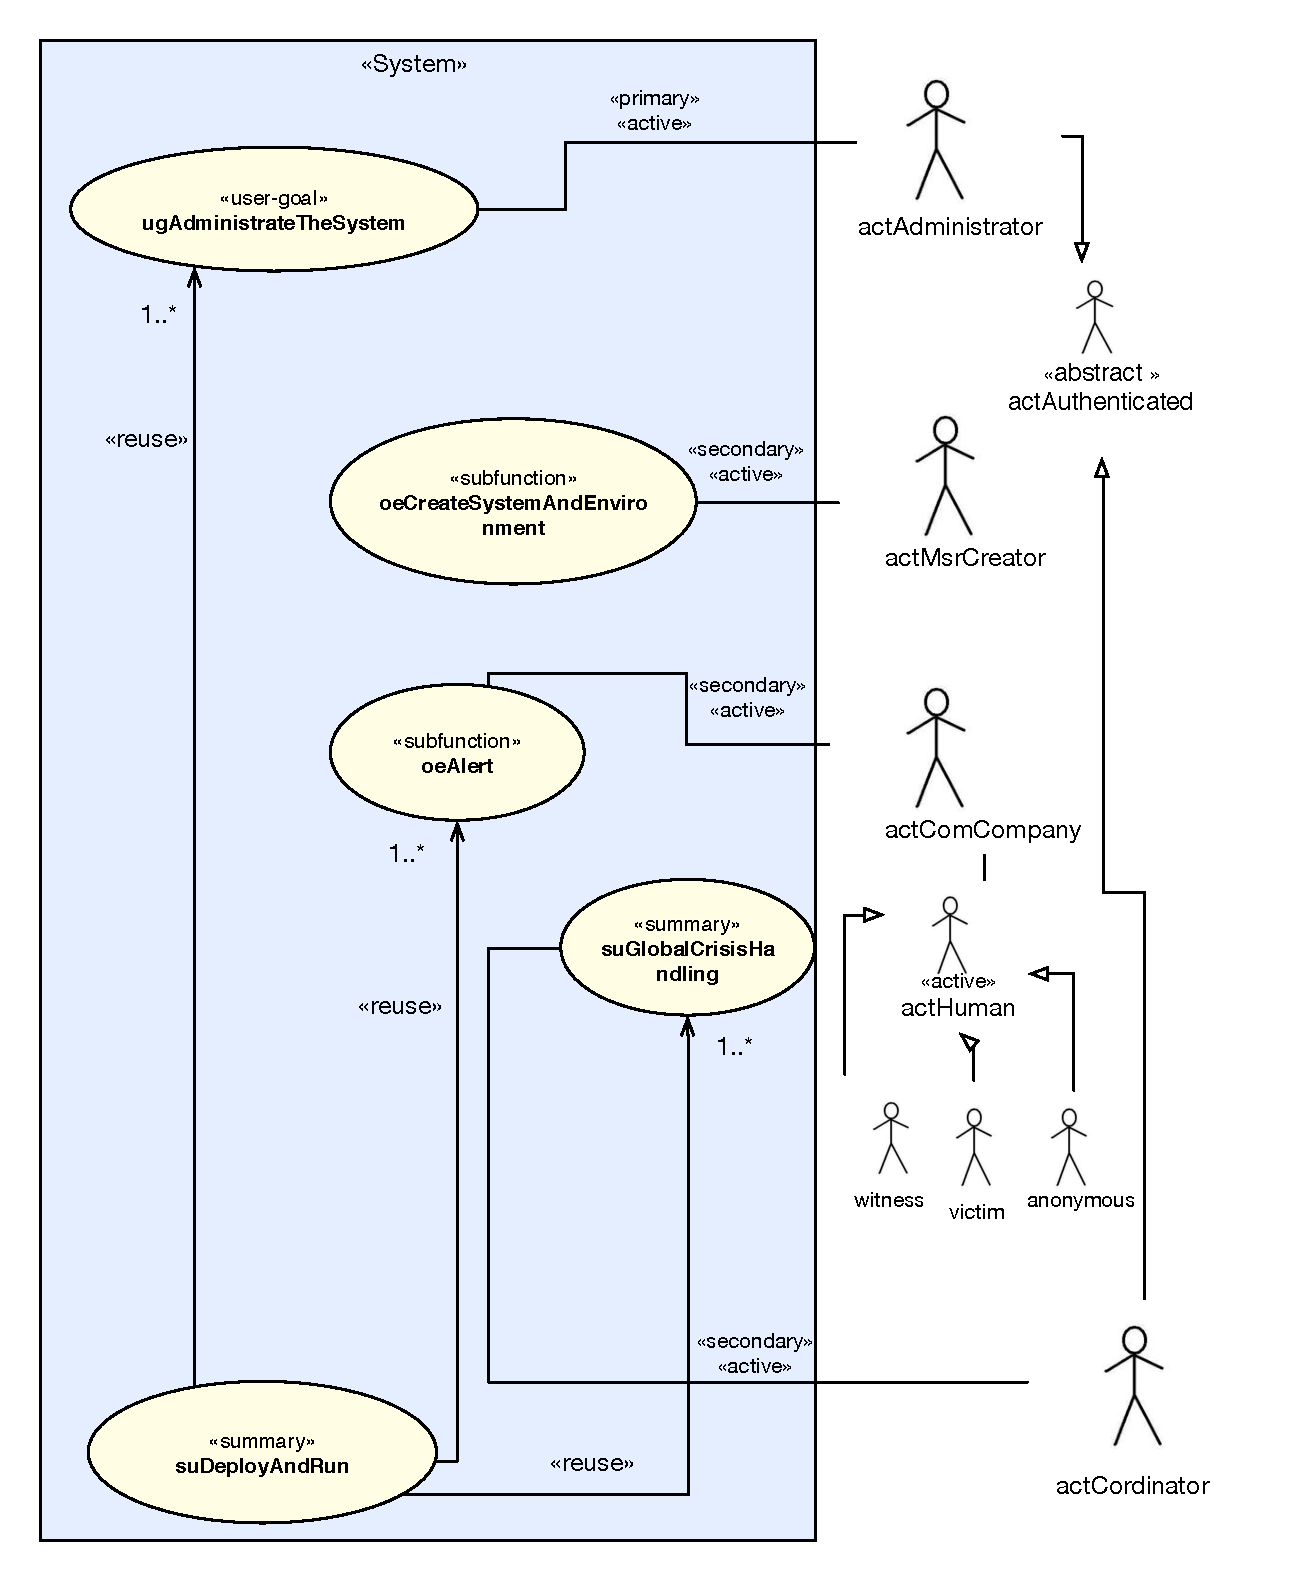
\includegraphics[width=150mm]{./images/suDeployAndRun.eps}
\normalsize}
\end{center}
\caption{\msricrash suDeployAndRun Use Case Diagram}
\label{fig:icrash-UCM-icrash-suDeployAndRun}
\end{figure}
\vspace{0.5cm}

\begin{figure}
\begin{center}
\scalebox{0.8}{
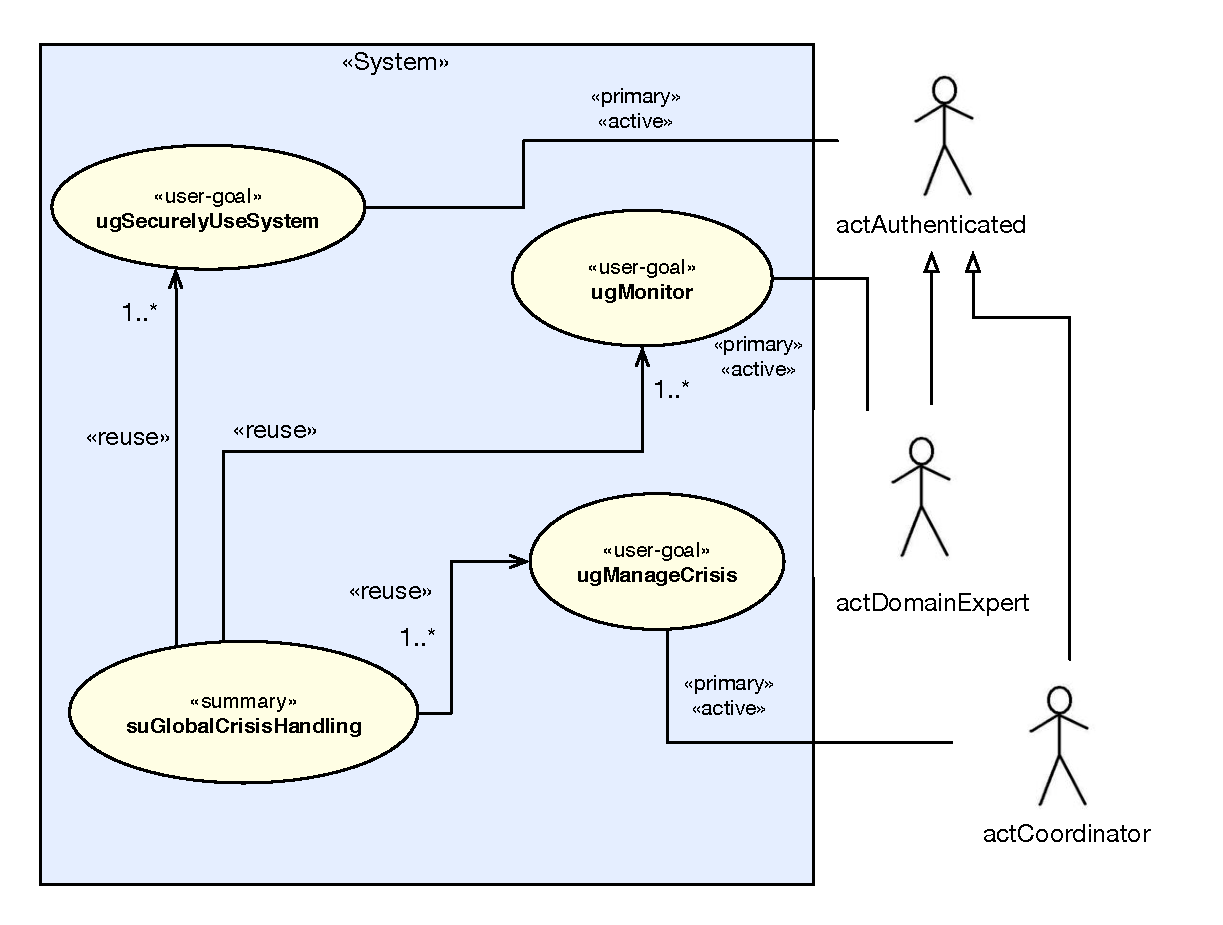
\includegraphics[width=150mm]{./images/ugGlobalCrisisHandling.eps}
\normalsize}
\end{center}
\caption{\msricrash suGlobalCrisisHandling Use Case Diagram}
\label{fig:icrash-UCM-icrash-suGlobalCrisisHandling}
\end{figure}
\vspace{0.5cm}

\begin{figure}
\begin{center}
\scalebox{0.8}{
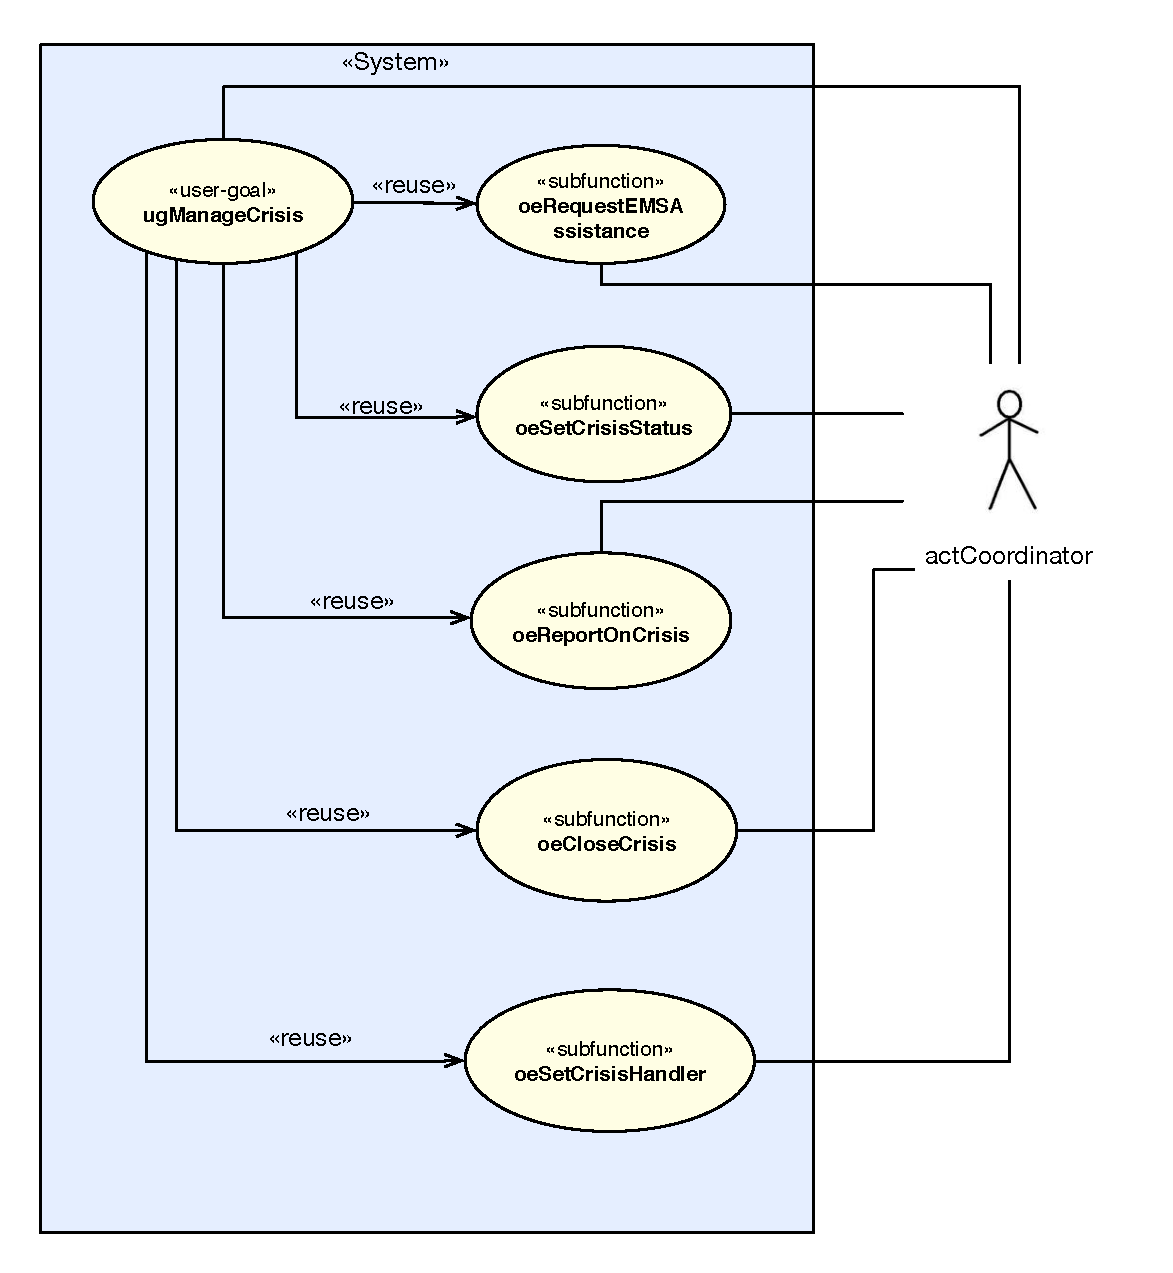
\includegraphics[width=150mm]{./images/UgManageCrisis.eps}
\normalsize}
\end{center}
\caption{\msricrash ugManageCrisis Use Case Diagram}
\label{fig:icrash-UCM-icrash-ugManageCrisis}
\end{figure}
\vspace{0.5cm}

\begin{figure}
\begin{center}
\scalebox{0.8}{
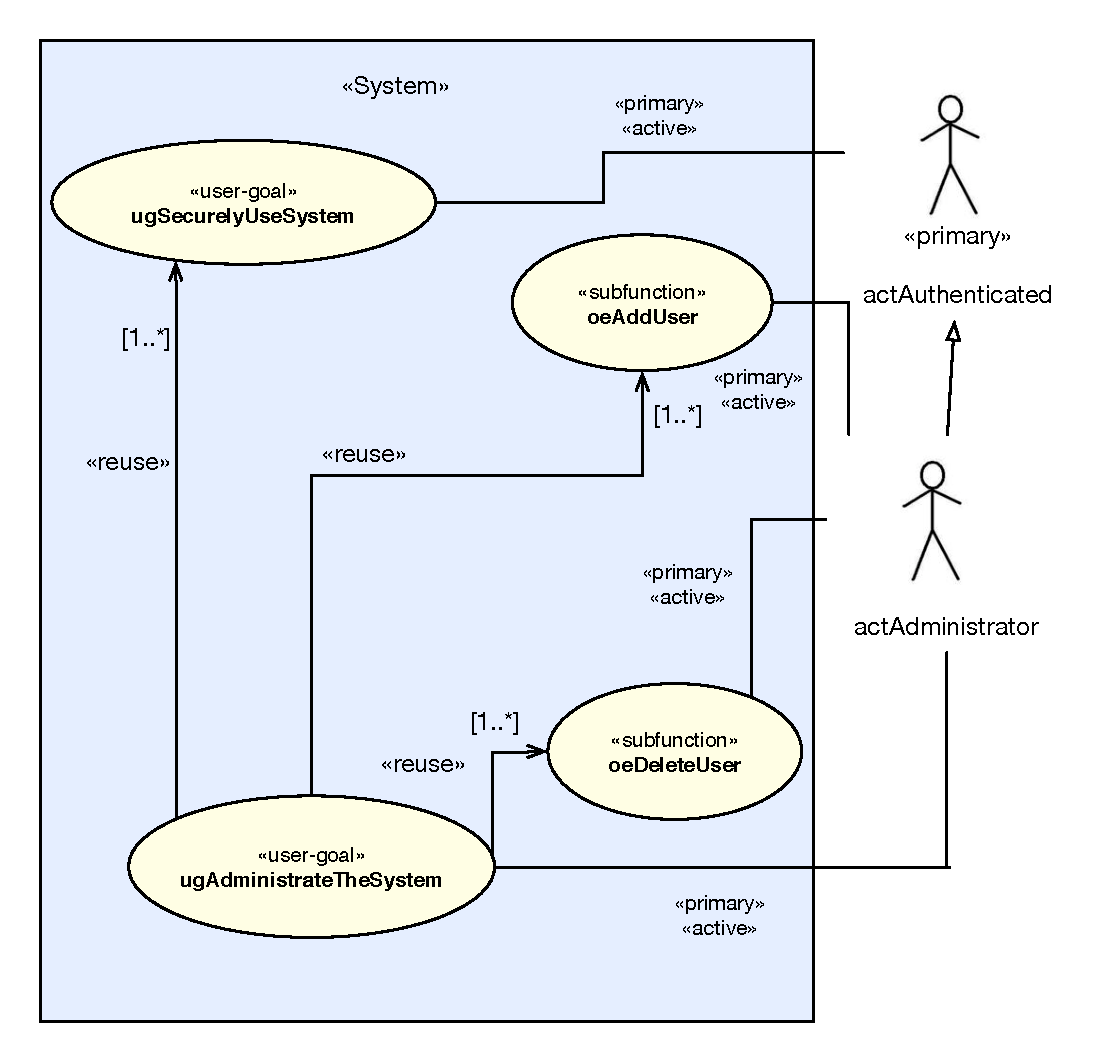
\includegraphics[width=150mm]{./images/ugAdministrateTheSystem.eps}
\normalsize}
\end{center}
\caption{\msricrash ugAdministrateTheSystem Use Case Diagram}
\label{fig:icrash-UCM-icrash-ugAdministrateTheSystem}
\end{figure}
\vspace{0.5cm}

\begin{figure}
\begin{center}
\scalebox{0.8}{
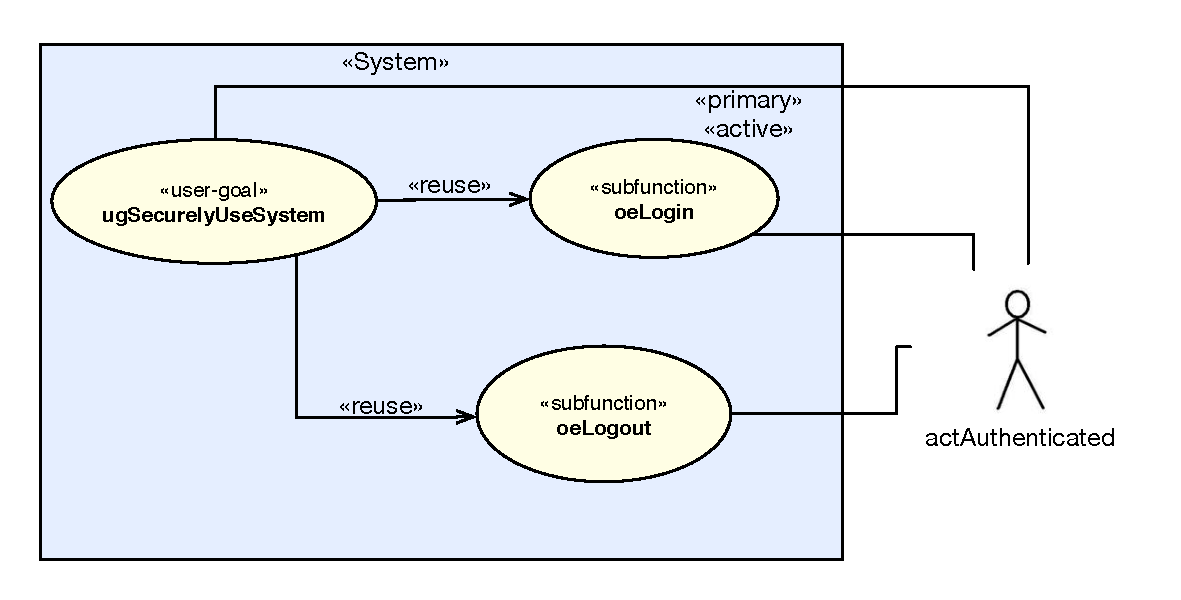
\includegraphics[width=150mm]{./images/ugSecurelyUseSystem.eps}
\normalsize}
\end{center}
\caption{\msricrash ugSecurelyUseSystem Use Case Diagram}
\label{fig:icrash-UCM-icrash-ugSecurelyUseSystem}
\end{figure}  
\vspace{0.5cm}

\begin{figure}
\begin{center}
\scalebox{0.8}{
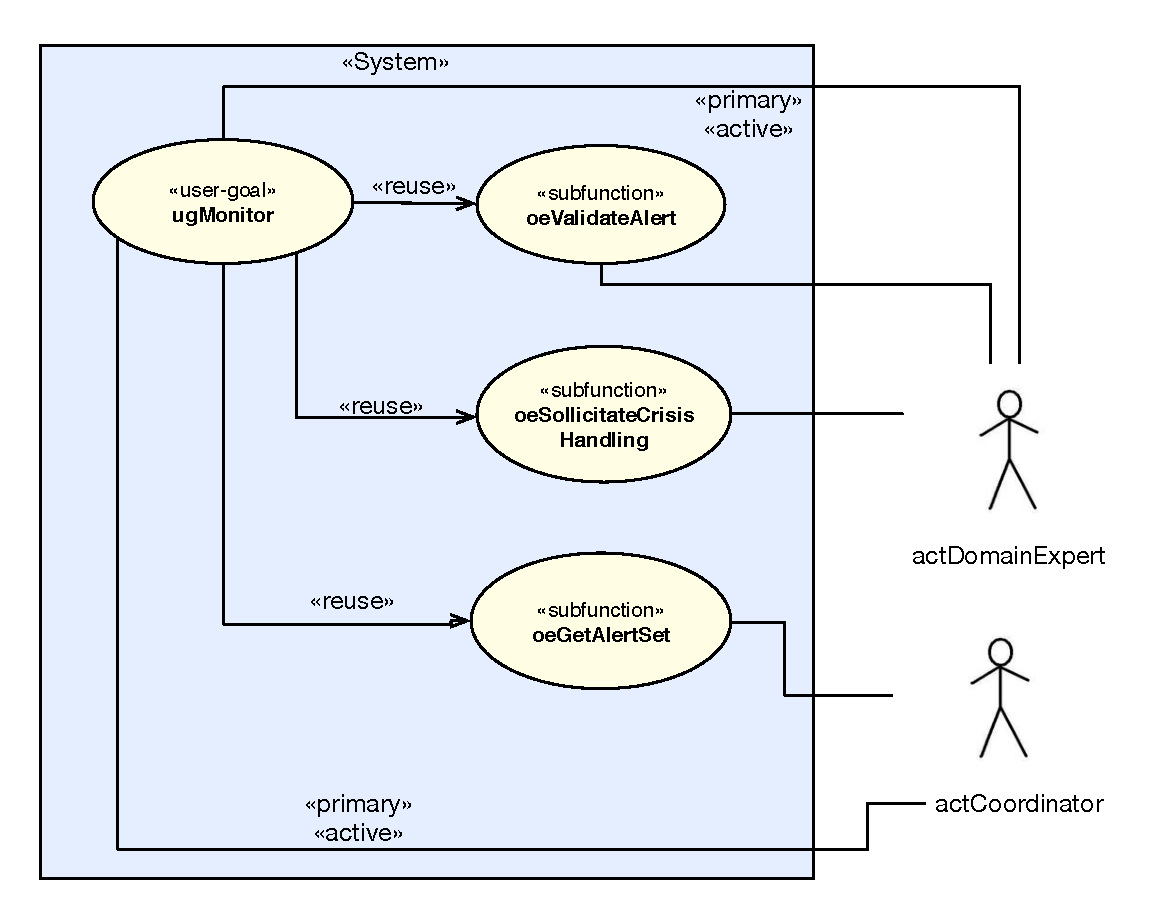
\includegraphics[width=150mm]{./images/UgMonitor.eps}
\normalsize}
\end{center}
\caption{\msricrash ugMonitor Use Case Diagram}
\label{fig:icrash-UCM-icrash-ugMonitor}
\end{figure}  
\vspace{0.5cm}

\clearpage

\subsection{Use Case Instance(s)}

The use case instance described below represents a summary level use case instance intended to illustrate a small and complete execution scenario of the \msricrash system. Figure \ref{fig:icrash-RE-UC-icrash-Test01-Communication-Diagram} provides informal graphical view (using a sequence diagram) of the messages sent during the scenario. The use case instance is described textually in the following use case description form as suggested by the \msrmessir method and inspired by the standard Cokburn template~\cite{armour01usecase}. We chose to indicate only messages sent by the environment to the system and not reply messages for readability.

\clearpage
\begin{usecaseinstance}
    \addheading{Use-Case Instance}
    \adddoublerow{Name}{Simple and Complete DeployAndRun Instance}
    \adddoublerow{Instance ID}{01}
    \adddoublerow{Environmental conditions and assumptions}{The necessary IT infrastructure exists to allow for deployment of the \msricrash system.}
    \adddoublerow{Inputs}{inputs are sequences of characters interpreted as string or numbers.}
    
    \addrowheading{Instance flow description}
    \addnumberedsinglerow{}{the \msrcode{actMsrCreator} actor \msrcode{theCreator} sends the message \msrcode{oeCreateSystemAndEnvironment(1)} requesting the initialization of the system and its environment (consisting of one administrator identified here by \msrcode{bill}) and indicating that the number of communication company actor instances for the system's environment is 1 (identified here by \msrcode{tango}).}
    \addnumberedsinglerow{}{the \msrcode{actAdministrator} actor \msrcode{bill} sends the message \msrcode{oeLogin(icrashadmin,7WXC1359)} to securely connect to the system.}
    \addnumberedsinglerow{}{the \msrcode{actAdministrator} actor \msrcode{bill} sends the message \msrcode{oeAddUser(1,Steve, pwdMessirExcalibur2017,1635242A75, 'Vehicular, Pedestrian, Wildlife, Property, Injury',Coordinator)} to set up a coordinator (i.e. identified here by \msrcode{steve}) and indicating his identification information, ID (i.e. \msrcode{1}) and a password (i.e. \msrcode{pwdMessirExcalibur2017}), id from a token(i.e.\msrcode{1635242A75}), specifying his domain of expertise(i.e. \msrcode{'Vehicular, Pedestrian, Wildlife, Property, Injury'}) and finally he designates the user as a Coordinator(i.e.\msrcode{Cooridnator}).}
    \addnumberedsinglerow{}{the \msrcode{actAdministrator} actor \msrcode{bill} sends the message \msrcode{oeAddUser(2, franklin, pwdMessirExcalibur, 1456872B82, Null, DomainExpert)} create a domain expert who is one person(i.e. identified here by \msrcode{franklin}) and indicating his user identification his identification, ID(i.e.\msrcode{2}), password(i.e.\msrcode{pwdMessirExcalibur123}), id from a token(i.e.\msrcode{14566872B82}), specifying the users domain of expertise as(\msrcode{Null} meaning that the user has no specific domain and can therefore only be an EMS user or Domain expert) and finally he designates the user as a domain expert(i.e.\msrcode{DomainExpert}).}
    \addnumberedsinglerow{}{the \msrcode{actAdministrator} actor \msrcode{bill} sends the message \msrcode{oeAddUser(3, barry, pwdEMSExcalibur321, 2436787C82, Null, EMS)} to set up a EMS user who is any user in the EMS headquarters(i.e. identified here by \msrcode{barry}) and indicating his user identification as ID(i.e.\msrcode{3}), password (i.e.\msrcode{pwdEMSExcalibur421}), id from a token(i.e.\msrcode{2436787C82}), specifying the users domain of expertise as(i.e.\msrcode{Null} meaning that the user has no specific domain and can therefore only be an EMS user or DomainExpert) and finally he designates the user as an EMS user(i.e.\msrcode{EMS}).}
    \addnumberedsinglerow{}{the \msrcode{actAdministrator} actor \msrcode{bill} sends the message \msrcode{oeLogout()} to disconnect from the system.}
    \addnumberedsinglerow{}{the \msrcode{actComCompany} actor \msrcode{tango} sends the message \msrcode{oeAlert(witness, 2017-11-26-at-10-10-16AM,+3524666445252, 49.627675-6.159590, '3 cars involved in an accident.')} to transfer a declaration of a car crash by a witness indicating specific phone number, the date and time, the GPS coordinates of the witnessed car crash and a short message giving additional details.}
    \addnumberedsinglerow{}{the \msrcode{actDomainExpert}actor \msrcode{franklin} sends the message \msrcode{oeLogin(franklin, pwdMessirExcalibur123, 687594FAD9)}to securely connect to the system entering his login(i.e.\msrcode{franklin}), his password(i.e.\msrcode{pwdMessirExcalibur123})and entering his serial key that he reads form a token device given to him by the administrator(i.e.687594FAD9).}
    \addnumberedsinglerow{}{the \msrcode{actEMS}actor \msrcode{barry} sends the message \msrcode{oeLogin(barry, pwdEMSExcalibur321, 24367872C282)}to securely connect to the system entering his login(i.e.\msrcode{barry}), his password(i.e.\msrcode{pwdEMSExcalibur321})and entering his serial key that he reads form a token device given to him by the administrator(i.e.\msrcode{24367872C282)}.}
    \addnumberedsinglerow{}{the \msrcode{actDomainExpert} actor \msrcode{franklin} sends the message \msrcode{oeValidateAlert(1,49.627675-6.159590,2017-11-26-at-10-10-16AM, valid, 'Vehicular, Pedestrian')}to validate the crisis and to set a Domain to it.}
    \addnumberedsinglerow{}{the \msrcode{actDomainExpert} actor \msrcode{franklin} sends the message \msrcode{oeSollicitateCrisisHandling()} indicating that there is a declared alert that is still not handled by any coordinator.}
    \addnumberedsinglerow{}{the \msrcode{actCoordinator} actor \msrcode{steve} sends the message \msrcode{oeLogin(steve, pwdMessirExcalibur2017, 63524275D9)} to securely connect to the system, entering his login(i.e.\msrcode{steve}), his password(i.e.\msrcode{pwdMessirExcalibur2017 }) and his serial Key that he reads form a token device he is given by the administrator(i.e.\msrcode{63524275D9})}
    \addnumberedsinglerow{}{the \msrcode{actCoordinator} actor \msrcode{steve} sends the message \msrcode{oeGetAlertsSet(valid)} to receive information about all the pending crisis.} \addnumberedsinglerow{}{the \msrcode{actCoordinator} actor \msrcode{steve} sends the message \msrcode{oeSetCrisisHandler(1,Medium, in-handling, 49.627095-6.160251, 2017-11-26-at-10-10-16AM)} to declare that he is taking care of the alert with the ID equal to \msrcode{1} which becomes the Crisis Id, sets the crisis type to(i.e.\msrcode{Medium}, the crisis type to(i.e.\msrcode{in-handling}), enters the GPS coordinates and the date and time.}
    \addnumberedsinglerow{}{the \msrcode{actComCompany} actor \msrcode{tango} sends the message \msrcode{oeAlert(witness, 2017-11-26-at-10-20-18AM,+3524666445314, 49.627095-6.160251,�Please send rescue services.�)} to transfer a declaration of a car crash by a witness indicating specific the phone number, the date and time, the GPS coordinates of the witnessed car crash and a short message giving additional details. This alert's GPS coordinates match the previous alert sent coordinates in step 7 and the time elapsed between the two alerts is 10 minutes therefore the alert is considered to be originating from the same location.}
    \addnumberedsinglerow{}{the \msrcode{actDomainExpert} actor \msrcode{franklin} sends the message \msrcode{oeValidateAlert(1,49.627675-6.159590,2017-11-26-at-10-10-16AM, valid, 'Vehicular, Pedestrian')}to validate the crisis and to set a Domain to it. Because the alert originated from the same location and only 10 min later it an automated message informs the Domain Expert to validate it to the same alert ID as the previous alert.}
    \addnumberedsinglerow{}{the \msrcode{actCoordinator} actor steve send the message \msrcode{oeReportOnCrisis(1, ' 2 Alerts received about a car accident at the same location apparently involving 3 vehicles', 2, Medium, Handled,'witness, 2017-11-26-at-10-10-16AM,+3524666445252, 49.627675-6.159590,'3 cars involved in an accident', witness, 2017-11-26-at-10-2-18AM,+3524666445314, 49.627095-6.160251,'Please send rescue services.',3, 3)} indicating the crisis ID(i.e.1), entering a specific comment in the comment area(i.e.\msrcode{'2Alertsrecived about a car accident at the same location apparently involving 3 vehicles'}), specifying his user ID(i.e.\msrcode{2}), setting the CrisisType(i.e.\msrcode{Medium}), indicating the current crisisStatus(\msrcode{handled}), entering the previous received alerts, indicating the number of vehicles involved in the accident(i.e.\msrcode{3}) and entering the number of victims(i.e.\msrcode{3}) because he suspects that there may be 3 victims due to the amount of cars involved in the accident. Entering a preliminary report on the crisis with the information that he presumes are right.}
    \addnumberedsinglerow{}{the \msrcode{actCoordinator} actor \msrcode {steve} send the message \msrcode{oeRequestEMSAssistance('We have received an Alert of an accident involving 3 cars from 1 victim and 1 witness at the same location please send police and ambulance',1, 49.627095-6.160251, 3,3, Ambulance Police)}, entering a comment(i.e. \msrcode{' We have received an Alert of an accident involving 3 cars from 1 victim and 1 witness at the same location please send Police assistance'}), indicating the RequestID(i.e.\msrcode{1}), entering the GPS location of the accident(i.e.\msrcode{49.627095-6.160251}), informing them of the number of cars involved(i.e.\msrcode{3}) and informing them of the presumed number of victims(i.e.\msrcode{3}) requesting emergency services assistance(i.e.\msrcode{Ambulance, Police}).}
    \addnumberedsinglerow{}{the \msrcode{actCooordinator} actor steve sends the message \msrcode{oeSetCrisisStatus(1, handled)}to change the status of the crisis identified by the ID(i.e.\msrcode{1}) to the status(i.e.\msrcode{handled}) thus indicating that he has handled the situation for now but it's not solved yet.}
    \addnumberedsinglerow{}{the \msrcode{actEMS} actor \msrcode{barry} sends the message \msrcode{oeReplyToRequest(1,'Message received, dispatching police and ambulance units.', 1, Handled)} indicating the CrisisID(i.e.\msrcode{1}), sending the comment(i.e.\msrcode{'Message received, dispatching police and ambulance units.'}), to confirm that the request with the ID(i.e.\msrcode{1}) has been received and is being handled, indicated by the EMS crisis status(i.e. \msrcode{Handled}).}
    \addnumberedsinglerow{}{the \msrcode{actEMS} actor \msrcode{barry} sends the message \msrcode{oeReportEMSCrisisStatus(1, 'Units arrived on scene report 4 victims, 3 cars involved in accident. Situation under control 1 victim brought Mercy hospital', solved, Mercy Hospital, Jeremy Springer, John Snow, +32168432)} indicating the crisis ID(i.e.\msrcode{1}), adding a comment(i.e. \msrcode{'Units arrived on scene report 4 victims, 3 cars involved in accident. Situation under control 1 brought to Mercy hospital'}), specifying the EMS crisis status as solved (i.e.\msrcode{solved}), indicating the hospital name as (i.e.\msrcode{Mercy Hospital}), indicating the victim name(i.e.\msrcode{Jeremy Springer}), indicating the victims ICE contact's name as(i.e.\msrcode{John Snow}) and the contacts phone number as (\msrcode{+32168432})  to report on the EMS crisis Status.}
    \addnumberedsinglerow{}{the \msrcode{actComCompany} actor \msrcode{tango} sends message \msrcode{oeInfoFam('Dear John Snow, I regret to inform you that Jeremy Springer was in a car accident involving 3 other cars. Jeremy Springer was brought to the Mercy hospital for examination. Regretfully yours..',Jeremy Springer, +32168432, Mercy Hospital)} to inform the victims family members about the state of the victim and in which hospital they reside.}
    \addnumberedsinglerow{}{the \msrcode{actCoordinator} actor \msrcode{steve} sends the message \msrcode{oeReportOnCrisis(1, ' 2 Alerts received about a car accident at the same location involving 3 vehicles and 4 victims one victim Jeremy Springer was brought to the Mercy hospital.', 2, Medium, Handled,'witness, 2017-11-26-at-10-10-16AM,+3524666445252, 49.627675-6.159590,'3 cars involved in an accident 'witness, 2017-11-26-at-10-2-18AM,+3524666445314, 49.627095-6.160251,'Please send rescue services.'',3, 4)} to set the report for the crisis with ID equal to 1 that he is handling.}
    \addnumberedsinglerow{}{the \msrcode{actCoordinator} actor \msrcode{steve} sends the message \msrcode{oeReportOnCrisis(1,'3 victims sent to hospital, 2 cars evacuated and 4 rescue unit mobilized')} to set the report for the crisis with \msrcode{ID} equal to 1 that he is handling.}
    \addnumberedsinglerow{}{the \msrcode{actCoordinator} actor \msrcode{steve} sends the message \msrcode{oeCloseCrisis(1)} to declare the crisis with ID equal to \msrcode{1} as closed.}
    \adddoublerow{Outputs}{at the end of this instance flow the system should have its environment made of one communication company actor instance, one coordinator actor instance, one administrator instance and the creator instance. The system state should contain two alerts defined according to the information received from the communication company, only one crisis that should be considered as solved and being alerted by the two alerts received.}
\end{usecaseinstance}

\clearpage

\begin{figure}[htbp]
\begin{center} 
\scalebox{0.95}{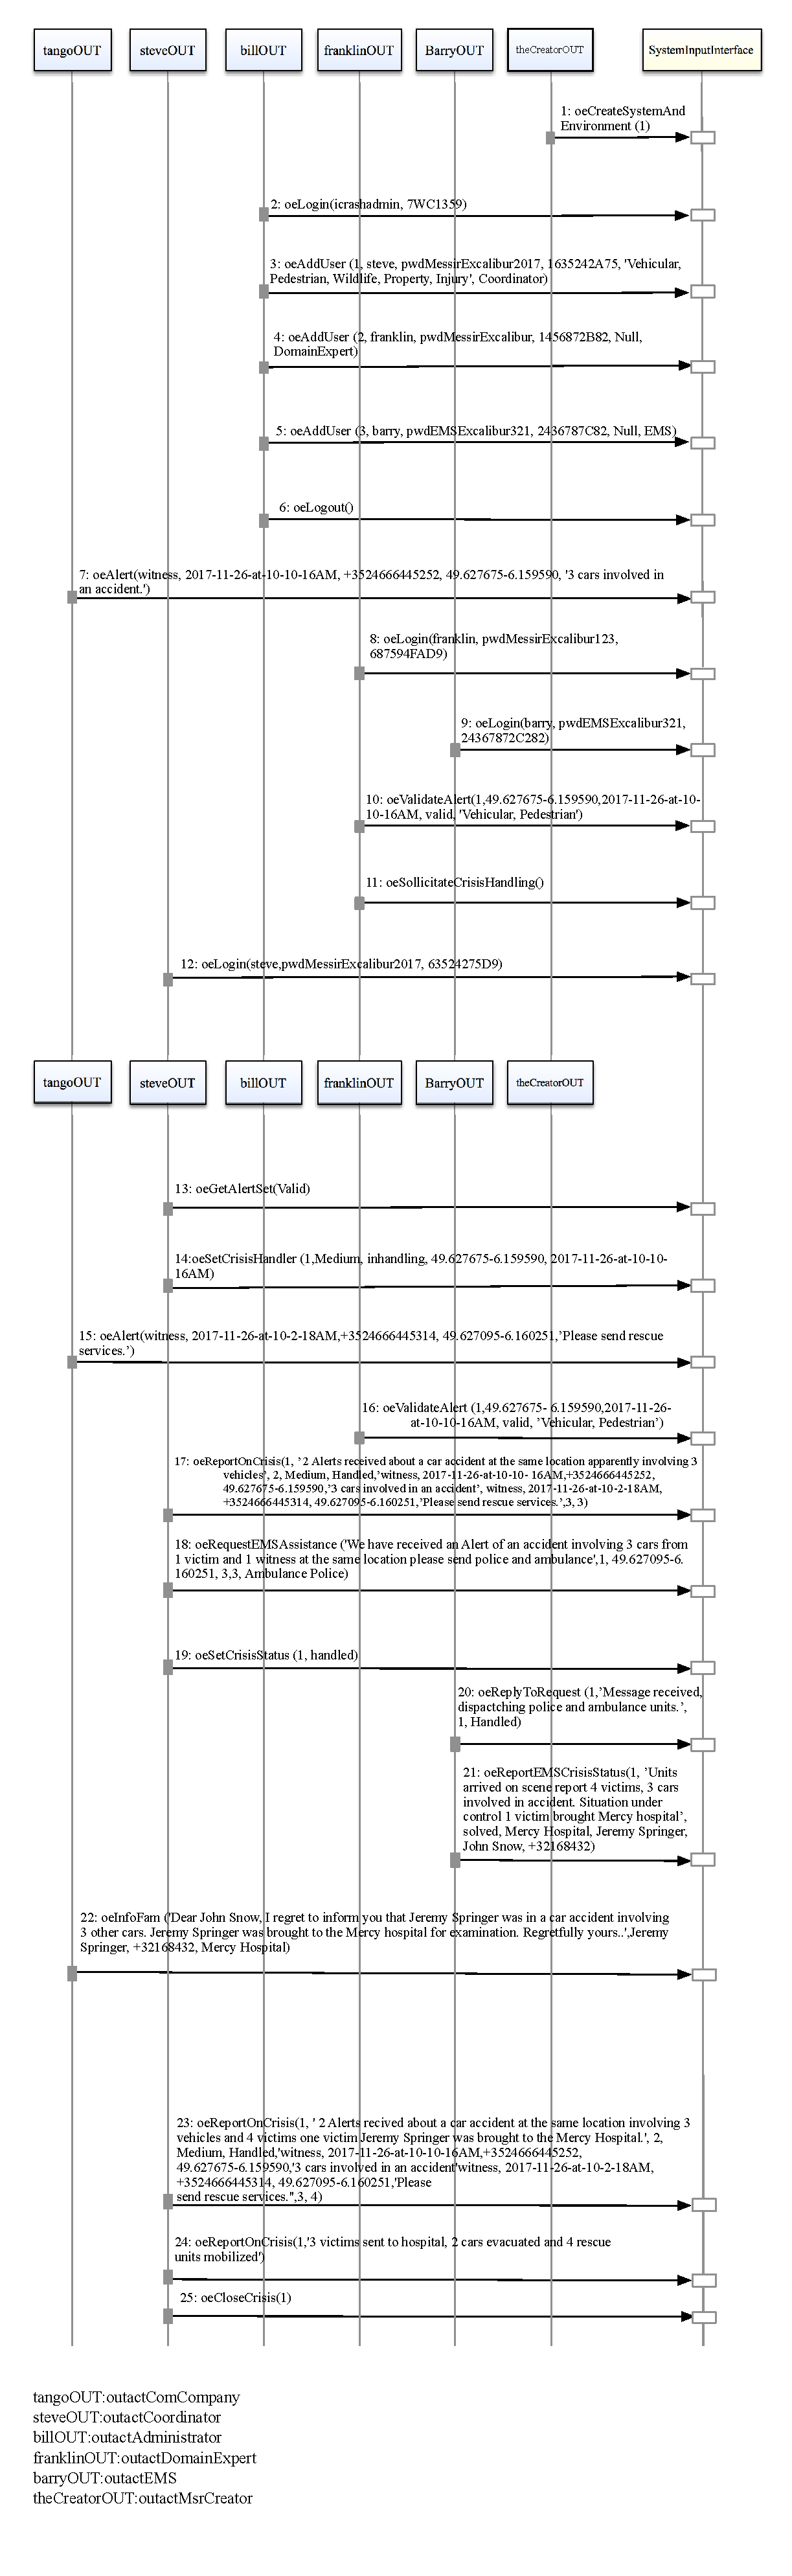
\includegraphics[width=180mm]{./images/SequenceDiagram.eps}\normalsize}
\end{center}
\caption[\msricrash Use Case Diagram:  SequenceDiagram Diagram]{\msricrash Use Case Diagram: SequenceDiagram}
\label{fig:icrash-RE-UCD-SequenceDiagram}
\end{figure}
\vspace{0.5cm}


